\documentclass[usenames,dvipsnames,aspectratio=169]{beamer}
\usepackage{../common/web}

\title[Web technológiák - CSS]{Web-technológia}
\subtitle{Cascading Style Sheets, II. rész}

\begin{document}

%1
\begin{frame}[plain]
  \titlepage
  \logoalul
\end{frame}

\section{CSS, 2. rész}

\subsection{Szövegformázás}

%53
\begin{frame}
  \begin{description}[m]
    \item[\texttt{text-align}] \hfill \\ Vízszintes igazítás: \texttt{left} (balra), \texttt{center} (középre), \texttt{right} (jobbra), \texttt{justify} (sorkizárt)
  \end{description}
  \begin{columns}[c]
    \column{0.6\textwidth}
      \begin{exampleblock}{\textattachfile{vizszintes.html}{vizszintes.html}}
        \tiny
        \lstinputlisting[style=HTML,linerange={7-10},numbers=left,firstnumber=7]{vizszintes.html}
        \lstinputlisting[style=HTML,linerange={15-16},numbers=left,firstnumber=15]{vizszintes.html}
      \end{exampleblock}
    \column{0.35\textwidth}
      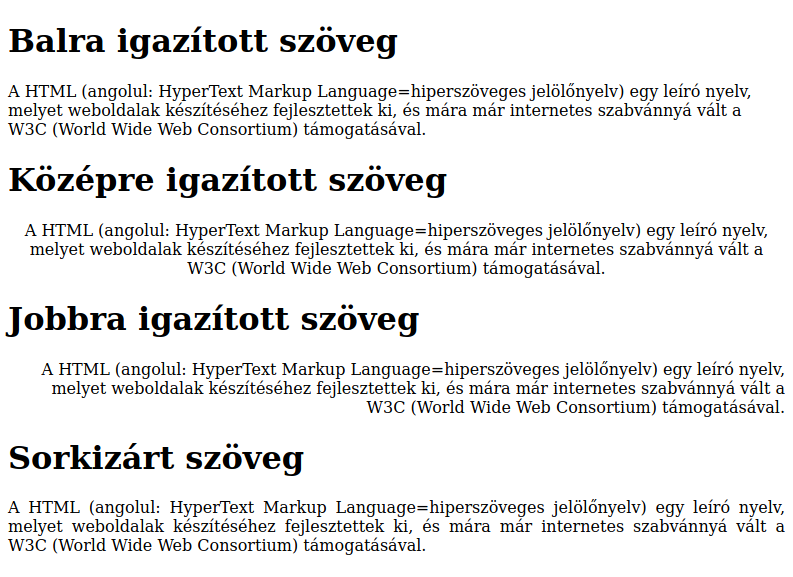
\includegraphics[width=\textwidth]{vizszintes.png}
  \end{columns}
\end{frame}

%54
\begin{frame}
  \texttt{hyphens}: elválasztások, hogy a szöveg tördelése még finomabb legyen
  \begin{description}[m]
    \item[\texttt{none}] \hfill \\ nincs elválasztás, alapértelmezés
    \item[\texttt{manual}] \hfill \\ elválasztás csak a kézzel előre megjelölt helyeken (\texttt{\&hyphen;}, \texttt{\&shy;})
    \item[\texttt{auto}] \hfill \\ automatikus elválasztás
  \end{description}
\end{frame}

%55
\begin{frame}
  \begin{exampleblock}{\textattachfile{elvalasztas.html}{elvalasztas.html}}
    \scriptsize
    \lstinputlisting[style=HTML,linerange={8-8},numbers=left,firstnumber=8]{elvalasztas.html}
    \lstinputlisting[style=HTML,linerange={12-13},numbers=left,firstnumber=12]{elvalasztas.html}
    \lstinputlisting[style=HTML,linerange={16-16},numbers=left,firstnumber=16]{elvalasztas.html}
  \end{exampleblock}
  \begin{center}
    
\includegraphics[width=\textwidth]{elvalasztas.png}
  \end{center}
\end{frame}

%56
\begin{frame}
  \texttt{vertical-align}: tetszőleges elem függőleges igazítása
  \begin{description}[m]
    \item[\texttt{baseline}] \hfill \\ szülő szövegének alapvonalához
    \item[\emph{távolság}] \hfill \\ tetszőleges mértékű süllyesztéshez/emeléshez, negatív érték is elfogadott
    \item[\texttt{\%}] \hfill \\ sormagasság \%-ában megadott emelés/süllyesztés, negatív érték is elfogadott
    \item[\texttt{sub}] \hfill \\ szülő alsó indexéhez
    \item[\texttt{super}] \hfill \\ szülő felső indexéhez
  \end{description}
\end{frame}

%57
\begin{frame}
  \begin{description}[m]
    \item[\texttt{top}] \hfill \\ sor legmagasabb eleméhez
    \item[\texttt{text-top}] \hfill \\ szülő elem szövegének tetejéhez
    \item[\texttt{middle}] \hfill \\ szülő közepéhez
    \item[\texttt{bottom}] \hfill \\  sor legalsó eleméhez
    \item[\texttt{text-bottom}] \hfill \\ szülő szövegének aljához
  \end{description}
\end{frame}

%58
\begin{frame}
  \begin{columns}[c]
    \column{0.55\textwidth}
      \begin{exampleblock}{\textattachfile{fuggoleges.html}{fuggoleges.html}}
        \tiny
        \lstinputlisting[style=HTML,linerange={7-9},numbers=left,firstnumber=7]{fuggoleges.html}
        \lstinputlisting[style=HTML,linerange={13-15},numbers=left,firstnumber=13]{fuggoleges.html}
      \end{exampleblock}
    \column{0.4\textwidth}
      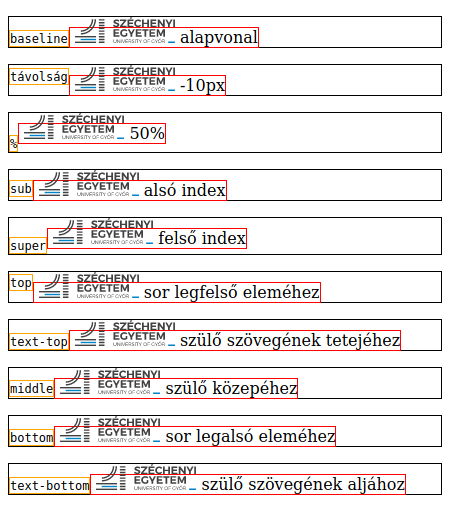
\includegraphics[width=\textwidth]{fuggoleges.png}
  \end{columns}
\end{frame}

%59
\begin{frame}
  \begin{description}[m]
    \item[\texttt{text-indent}] \hfill \\ Első sor behúzása: \emph{távolság} (a bekezdés bal szélétől számított behúzás), \texttt{\%} (szülő elem szélességének százalékában adott behúzás)
  \end{description}
  \begin{columns}[c]
    \column{0.6\textwidth}
      \begin{exampleblock}{\textattachfile{behuzas.html}{behuzas.html}}
        \tiny
        \lstinputlisting[style=HTML,linerange={7-10},numbers=left,firstnumber=7]{behuzas.html}
        \lstinputlisting[style=HTML,linerange={14-16},numbers=left,firstnumber=14]{behuzas.html}
      \end{exampleblock}
    \column{0.35\textwidth}
      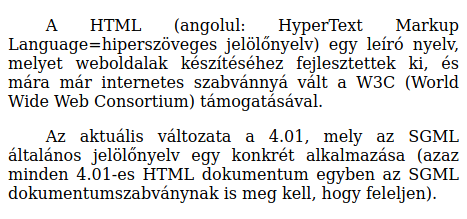
\includegraphics[width=\textwidth]{behuzas.png}
  \end{columns}
\end{frame}

%60
\begin{frame}
  \texttt{white-space}: fehér karakterek értelmezése
  \begin{description}[m]
    \item[\texttt{normal}] \hfill \\ szomszédos fehér karaktereket összevonja, alapértelmezés
    \item[\texttt{nowrap}] \hfill \\ nem tördeli a hosszú sorokat, de a szomszédos fehér karaktereket összevonja
    \item[\texttt{pre}] \hfill \\ utánozza a \texttt{<pre>} HTML elem működését, minden fehér karaktert megőriz
    \item[\texttt{pre-line}] \hfill \\ szomszédos fehér karaktereket összevonja, de tördeli a sorokat, ha szükséges
    \item[\texttt{pre-wrap}] \hfill \\ minden fehér karaktert megőriz, és tördel, ha szükséges
  \end{description}
\end{frame}

%61
\begin{frame}
  Nem választ magától \texttt{monospace} karakterkészletet!
  \begin{columns}[c]
    \column{0.6\textwidth}
      \begin{exampleblock}{\textattachfile{fahrcels2.html}{fahrcels2.html}}
        \footnotesize
        \lstinputlisting[style=HTML,linerange={7-10},numbers=left,firstnumber=7]{fahrcels2.html}
        \lstinputlisting[style=HTML,linerange={14-16},numbers=left,firstnumber=14]{fahrcels2.html}
      \end{exampleblock}
    \column{0.35\textwidth}
      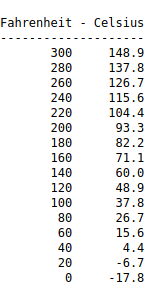
\includegraphics[width=0.7\textwidth]{fahrcels2.png}
  \end{columns}
\end{frame}

%62
\begin{frame}
  \texttt{letter-spacing}: betűk közötti távolság
  \begin{description}[m]
    \item[\texttt{normal}] \hfill \\ szokásos távolság, alapértelmezés
    \item[\emph{távolság}] \hfill \\ betűk közötti távolság, negatív érték is elfogadott
  \end{description}
  \vfill
  \texttt{word-spacing}: szavak közötti távolság
  \begin{description}[m]
    \item[\texttt{normal}] \hfill \\ szokásos távolság (betűmagasság negyede), alapértelmezés
    \item[\emph{távolság}] \hfill \\ szavak közötti távolság, negatív érték is elfogadott
  \end{description}
\end{frame}

%63
\begin{frame}
  \begin{exampleblock}{\textattachfile{tavolsag.html}{tavolsag.html}}
    \footnotesize
    \lstinputlisting[style=HTML,linerange={7-11},numbers=left,firstnumber=7]{tavolsag.html}
    \lstinputlisting[style=HTML,linerange={15-16},numbers=left,firstnumber=15]{tavolsag.html}
  \end{exampleblock}
  \begin{center}
    
\includegraphics[width=0.8\textwidth]{tavolsag.png}
  \end{center}
\end{frame}

%64
\begin{frame}
  \texttt{text-transform}: szöveg átalakítása
  \begin{description}[m]
    \item[\texttt{normal}] \hfill \\ nincs átalakítás, alapértelmezés
    \item[\texttt{capitalize}] \hfill \\ minden kezdőbetűt nagybetűvel nyomtat
    \item[\texttt{uppercase}] \hfill \\ csupa nagybetűvel nyomtat
    \item[\texttt{lowercase}] \hfill \\ csupa kisbetűvel nyomtat
  \end{description}
\end{frame}

%65
\begin{frame}
  \begin{exampleblock}{\textattachfile{nagybetu.html}{nagybetu.html}}
    \scriptsize
    \lstinputlisting[style=HTML,linerange={7-9},numbers=left,firstnumber=7]{nagybetu.html}
    \lstinputlisting[style=HTML,linerange={13-14},numbers=left,firstnumber=13]{nagybetu.html}
  \end{exampleblock}
  \begin{center}
    
\includegraphics[scale=0.5]{nagybetu.png}
  \end{center}
\end{frame}

%66
\begin{frame}
  \texttt{text-decoration-line}: vonal húzása a szöveggel párhuzamosan
  \begin{description}[m]
    \item[\texttt{none}] \hfill \\ nincs vonalazás, alapértelmezés. Pl. hivatkozások aláhúzásának eltávolításához használható.
    \item[\texttt{underline}] \hfill \\ aláhúzza a szöveget; \kiemel{félrevezetheti az olvasót}, ha nem csak a hivatkozások jelennek meg aláhúzással!
    \item[\texttt{overline}] \hfill \\ a szöveg fölött húz vonalat
    \item[\texttt{line-through}] \hfill \\ áthúzza a szöveget
  \end{description}
\end{frame}

%67
\begin{frame}
  \texttt{text-decoration-style}: a vonal stílusa
  \begin{description}[m]
    \item[\texttt{solid}] \hfill \\ folytonos vonal
    \item[\texttt{double}] \hfill \\ dupla vonal
    \item[\texttt{dotted}] \hfill \\ pontvonal
    \item[\texttt{dashed}] \hfill \\ szaggatott vonal
    \item[\texttt{wavy}] \hfill \\ hullámos vonal
  \end{description}
\end{frame}

%68
\begin{frame}
  \texttt{text-decoration-color}: a vonal színe
  \begin{description}[m]
    \item[\emph{szín}] \hfill \\ tetszőleges CSS színmegadási móddal
  \end{description}
  \vfill
  Rövidítés:
  \begin{description}[m]
    \item[\texttt{text-decoration:}]
    \item[\qquad\texttt{text-decoration-line text-decoration-color text-decoration-style}] \hfill \\ Akár többféle vonal is megadható, tetszőleges rész elhagyható, sorrend tetszőleges
  \end{description}
\end{frame}

%69
\begin{frame}
  \begin{exampleblock}{\textattachfile{dekoracio.html}{dekoracio.html}}
    \footnotesize
    \lstinputlisting[style=HTML,linerange={7-11},numbers=left,firstnumber=7]{dekoracio.html}
    \lstinputlisting[style=HTML,linerange={15-17},numbers=left,firstnumber=15]{dekoracio.html}
  \end{exampleblock}
  \begin{center}
    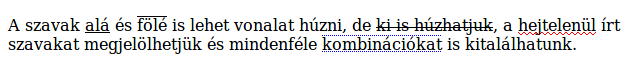
\includegraphics[width=\textwidth]{dekoracio.png}
  \end{center}
\end{frame}

%70
\begin{frame}
  \texttt{text-shadow}: szöveg árnyéka
  \begin{description}[m]
    \item[\texttt{h-shadow v-shadow blur-radius color}] \hfill \\ vízszintes eltolás, függőleges eltolás, elmosás mértéke, szín. \\ Az elmosás mértéke elhagyható, a többi kötelező. Az eltolásoknál negatív értékek megengedettek. Vesszővel elválasztva több árnyék is megadható egyszerre.
    \item[\texttt{none}] nincs árnyék, alapértelmezés
  \end{description}
\end{frame}

%71
\begin{frame}
  \begin{columns}[c]
    \column{0.7\textwidth}
      \begin{exampleblock}{\textattachfile{arnyek.html}{arnyek.html}}
        \scriptsize
        \lstinputlisting[style=HTML,linerange={7-12},numbers=left,firstnumber=7]{arnyek.html}
        \lstinputlisting[style=HTML,linerange={16-18},numbers=left,firstnumber=16]{arnyek.html}
      \end{exampleblock}
    \column{0.25\textwidth}
      
\includegraphics[width=\textwidth]{arnyek.png}
  \end{columns}
\end{frame}

%72
\begin{frame}
  \texttt{line-height}: sormagasság
  \begin{description}[m]
    \item[\texttt{normal}] \hfill \\ betűméretből következő sormagasság, alapértelmezett
    \item[\emph{szám}] \hfill \\ az aktuális betűméretet ezzel szorozva kapja meg a sormagasságot
    \item[\emph{távolság}] \hfill \\ rögzített sormagasság, CSS mértékegységben
    \item[\texttt{\%}] \hfill \\ az aktuális betűméret \%-a
  \end{description}
\end{frame}

%73
\begin{frame}
  \begin{columns}[c]
    \column{0.65\textwidth}
      \begin{exampleblock}{\textattachfile{sormagassag.html}{sormagassag.html}}
        \scriptsize
        \lstinputlisting[style=HTML,linerange={7-9},numbers=left,firstnumber=7]{sormagassag.html}
        \lstinputlisting[style=HTML,linerange={13-15},numbers=left,firstnumber=13]{sormagassag.html}
      \end{exampleblock}
    \column{0.3\textwidth}
      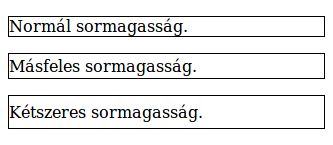
\includegraphics[width=\textwidth]{sormagassag.png}
  \end{columns}
\end{frame}

%74
\begin{frame}
  Többféle írásirány támogatott egyazon oldalon
  \begin{columns}[c]
    \column{0.65\textwidth}
      \begin{exampleblock}{\textattachfile{irasirany.html}{irasirany.html}}
        \footnotesize
        \lstinputlisting[style=HTML,linerange={7-10},numbers=left,firstnumber=7]{irasirany.html}
        \lstinputlisting[style=HTML,linerange={14-15},numbers=left,firstnumber=14]{irasirany.html}
      \end{exampleblock}
    \column{0.3\textwidth}
      
\includegraphics[width=\textwidth]{irasirany.png}
  \end{columns}  
\end{frame}

%75
\begin{frame}
  \begin{columns}[c]
    \column{0.5\textwidth}
      \footnotesize
      Készítse el az ábrán látható weboldalt!
      \begin{itemize}
        \item Induljon ki a \textattachfile{szoveg.txt}{szoveg.txt} fájlból!
        \item A címsor betűi között hagyjon 5-5 képpontnyi helyet,
        \item írja csupa nagybetűvel, és
        \item jelenítsen meg alatta 3-3 képpontnyival jobbra és lefelé eltolt árnyékot, mely kék színű, és elmosásának sugara 10 képpont!
        \item A bekezdés legyen sorkizárt igazítású, 
        \item a sormagasság másfélszeres,
        \item az első sor behúzása 20 képpontnyi,
        \item és automatikusan elválasztott!
        \item Az emberek neveit emelje ki zöld színű, dupla aláhúzással!
      \end{itemize}
    \column{0.45\textwidth}
      \begin{exampleblock}{\textattachfile{szoveg.html}{szoveg.html}}
        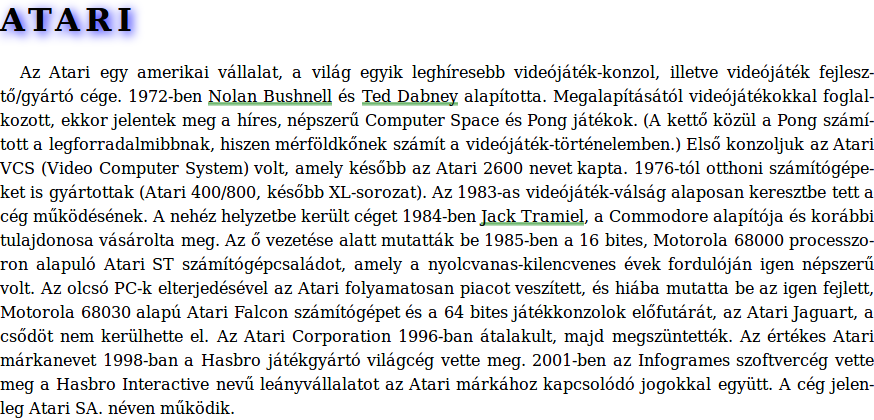
\includegraphics[width=\textwidth]{szoveg.png}
      \end{exampleblock}
  \end{columns}
\end{frame}

\subsection{Ikonok}

%_
\begin{frame}
  Ikonok:
  \begin{itemize}
    \item feldobják az oldal megjelenését
    \item lényegretörő, kifejező
  \end{itemize}
  \vfill
  Használat: \texttt{<i>} vagy \texttt{<span>} elemek + \texttt{class} attribútum
  \vfill
  CSS-sel formázhatóak: méret, szín, árnyék, szegély, stb.
  \vfill
  Több ikon könyvtár is elérhető.
\end{frame}

%_
\begin{frame}
  \hiv{\href{https://fontawesome.com}{Font Awesome}}
  \begin{itemize}
    \item 1588 ikon ingyen + 7842 fizetős
    \item Kit kódot kell igényelni a használathoz (az enyém pl. 5e6bd4a2fc)
    \item Egy \texttt{<script>} elemet kell beszúrni az oldalba a használathoz
    \item \texttt{class} attribútum értékei az ikonkészlet választáshoz:
    \begin{itemize}
      \item \texttt{fas} $\to$ Font Awesome Solid
      \item \texttt{fab} $\to$ Font Awesome Brand
      \item \texttt{Regular}, \texttt{Light}, \texttt{Duotone} a fizetős változatban
    \end{itemize}
    \item \texttt{class} attribútum értékei méretezéshez (enélkül a betűmérethez igazodik):
    \begin{itemize}
      \item \texttt{fa-xs}, \texttt{fa-sm}, \texttt{fa-lg}
      \item \texttt{fa-2x}, \texttt{fa-3x}, \dots, \texttt{fa-10x}
    \end{itemize}
  \end{itemize}
\end{frame}

%
\begin{frame}
  \begin{itemize}
    \item Léteznek azonos szélességű ikonok, pl. függőlegesen elrendezett menühöz (\texttt{fa-fw})
    \item Felsorolásjelekként állhatnak (pl. \texttt{fa-ul}, \texttt{fa-li}, \texttt{fa-check-square})
    \item Forgathatóak, tükrözhetőek (pl. \texttt{fa-rotate-90}, \texttt{fa-flip-vertical})
    \item Animálhatóak (\texttt{fa-spin}, \texttt{fa-pulse})
    \item Fizetős változat további szolgáltatásokkal: méretezés, pozicionálás, maszkolás, rétegek, \dots
    \item Egy lehetséges alternatíva: \hiv{\href{https://icons8.com/line-awesome}{Line Awesome}}
  \end{itemize}
\end{frame}

%_
\begin{frame}
  \begin{columns}[c]
    \column{0.76\textwidth}
      \begin{exampleblock}{\textattachfile{fontawesome.html}{fontawesome.html}}
        \scriptsize
        \lstinputlisting[style=HTML,linerange={7-8},numbers=left,firstnumber=7]{fontawesome.html}
        \lstinputlisting[style=HTML,linerange={12-23},numbers=left,firstnumber=12]{fontawesome.html}
      \end{exampleblock}
    \column{0.2\textwidth}
      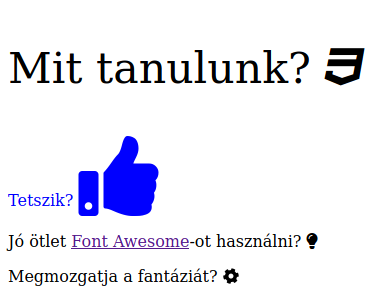
\includegraphics[width=\textwidth]{fontawesome.png}
  \end{columns}
\end{frame}

%_
\begin{frame}
  Google Material Icons
  \begin{itemize}
    \item Egységes, letisztult UI készítéséhez használható ikonkészlet, és UI tervezési elvek
    \item Kevesebb ikon, egyszerűbb szolgáltatások, ligatúrákat használ.
    \item \hiv{\href{https://material.io/resources/icons}{Ikonlista}}
    \item \hiv{\href{https://google.github.io/material-design-icons/}{Felhasználási útmutató}}
    \item Egy stíluslap betöltése után használható
    \item Az oldal szerkesztőjének kell stílusokat definiálni a méretezéshez (pl. \texttt{md-48}), színezéshez (pl. \texttt{md-dark}), stb.
  \end{itemize}
\end{frame}

%_
\begin{frame}
  \begin{columns}[c]
    \column{0.76\textwidth}
      \begin{exampleblock}{\textattachfile{material.html}{material.html}}
        \scriptsize
        \lstinputlisting[style=HTML,linerange={6-12},numbers=left,firstnumber=6]{material.html}
        \lstinputlisting[style=HTML,linerange={24-29},numbers=left,firstnumber=24]{material.html}
      \end{exampleblock}
    \column{0.2\textwidth}
      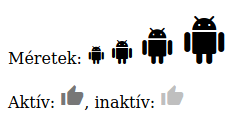
\includegraphics[width=\textwidth]{material.png}
  \end{columns}
\end{frame}

\subsection{Hivatkozások}

%_
\begin{frame}
  A \emph{látszólagos osztály} (pseudo class) egy, a szelektor utáni 
  :-ot követő kulcsszó, amivel a kiválasztott elem(ek) különféle 
  állapotaiban alkalmazandó formázás adható meg.\\
  \vfill
  \hiv{\href{https://developer.mozilla.org/en-US/docs/Web/CSS/Pseudo-classes}{Látszólagos osztályok referenciája}}
  \vfill
  Hivatkozásoknál alkalmazható:
  \begin{description}[m]
    \item[\texttt{link}] \hfill \\ Még nem követték a hivatkozást
    \item[\texttt{visited}] \hfill \\ Már követték a hivatkozást
    \item[\texttt{hover}] \hfill \\ Egér a hivatkozás felett
    \item[\texttt{active}] \hfill \\ Már rákattintottak, de az új 
    tartalom még nem töltődött be
  \end{description}
  \kiemel{Ebben a sorrendben} kell definiálni őket!
\end{frame}

%
\begin{frame}
  \begin{exampleblock}{\textattachfile{hivatkozas.html}{hivatkozas.html}}
    \scriptsize
    \lstinputlisting[style=HTML,linerange={7-10},numbers=left,firstnumber=7]{hivatkozas.html}
    \lstinputlisting[style=HTML,linerange={14-16},numbers=left,firstnumber=14]{hivatkozas.html}
  \end{exampleblock}
  \begin{center}
    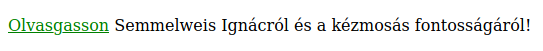
\includegraphics[width=0.8\textwidth]{hivatkozas.png}
  \end{center}
\end{frame}

\subsection{Egérkurzor alakja}

%_
\begin{frame}
  \begin{columns}[c]
    \column{0.8\textwidth}
      \begin{itemize}
        \item Rengeteg előre beépített egérkurzor közül lehet választani a \texttt{cursor} tulajdonság értékének állításával.
        \item Saját kurzort is lehet betölteni az \texttt{url()} függvénnyel, de célszerű utána vesszővel elválasztva egy beépített kurzort is megnevezni, betöltési hiba esetére.
        \item Kurzor akár \hiv{\href{https://www.cursor.cc/}{online}} is szerkeszthető.
      \end{itemize}
    \column{0.15\textwidth}
      \begin{exampleblock}{\textattachfile{kurzor.html}{kurzor.html}, \textattachfile{cursor.cur}{cursor.cur}}
        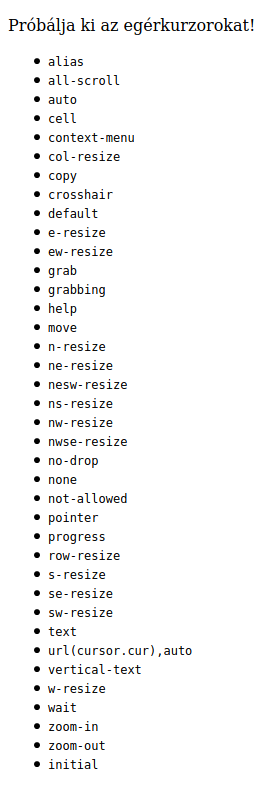
\includegraphics[width=.8\textwidth]{kurzor.png}
      \end{exampleblock}
  \end{columns}
\end{frame}

\subsection{Felsorolások}

%
\begin{frame}
  \begin{description}[m]
    \item[\texttt{list-style-type}] \hfill \\ Felsorolásjel típusa\\
    \begin{itemize}
      \item Számozott listákhoz, pl. \texttt{decimal} (arab számok), \texttt{lower-alpha} (kisbetűk), \texttt{upper-roman} (római számok nagybetűkkel)
      \item Nem számozott listákhoz, pl. \texttt{disc} (körlemez), \texttt{circle} (körvonal), \texttt{square} (négyzet)
      \item Eltüntetés: \texttt{none}
    \end{itemize}
  \end{description}
\end{frame}

%
\begin{frame}
  \begin{columns}[c]
    \column{0.45\textwidth}
      \begin{exampleblock}{\textattachfile{szamozott.html}{szamozott.html}}
        \begin{center}
          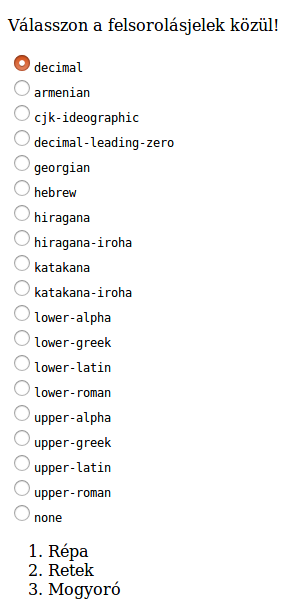
\includegraphics[width=.37\textwidth]{szamozott.png}
        \end{center}
      \end{exampleblock}
    \column{0.45\textwidth}
      \begin{exampleblock}{\textattachfile{nemszamozott.html}{nemszamozott.html}}
        \begin{center}
          
\includegraphics[width=.7\textwidth]{nemszamozott.png}
        \end{center}
      \end{exampleblock}
  \end{columns} 
\end{frame}

%
\begin{frame}
  \begin{columns}[c]
    \column{0.7\textwidth}
      \begin{description}[m]
        \item[\texttt{list-style-image}] \hfill \\ A felsorolásjel egy kép \texttt{url()} függvénnyel, vagy \texttt{none}.\\
        Érdemes megadni a \texttt{list-style-type}-ot is, hátha nem lehet megjeleníteni a képet.
      \end{description}
      \vfill
      \begin{exampleblock}{\textattachfile{sajatjelolo.html}{sajatjelolo.html}}
        \scriptsize
        \lstinputlisting[style=HTML,linerange={7-7},numbers=left,firstnumber=7]{sajatjelolo.html}
      \end{exampleblock}
    \column{0.25\textwidth}
      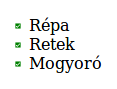
\includegraphics[width=\textwidth]{sajatjelolo.png}
  \end{columns} 
\end{frame}

%
\begin{frame}
  \begin{columns}[c]
    \column{0.7\textwidth}
      \begin{description}[m]
        \item[\texttt{list-style-position}] \hfill \\ A felsorolásjel helyzete\\
        \begin{itemize}
          \item \texttt{outside}: a bekezdés bal széle előtt, alapértelmezés.
          \item \texttt{inside}: a bekezdésen belül, a szöveg részeként.
        \end{itemize}
      \end{description}
      \vfill
      \begin{exampleblock}{\textattachfile{kivulbelul.html}{kivulbelul.html}}
        \scriptsize
        \lstinputlisting[style=HTML,linerange={7-9},numbers=left,firstnumber=7]{kivulbelul.html}
      \end{exampleblock}
    \column{0.25\textwidth}
      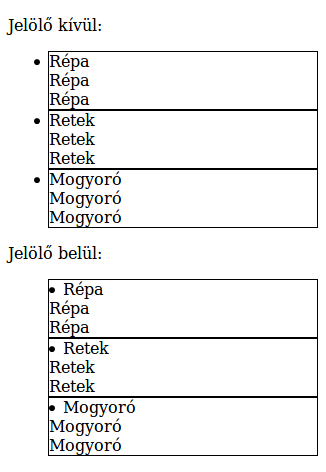
\includegraphics[width=\textwidth]{kivulbelul.png}
  \end{columns} 
\end{frame}

%
\begin{frame}
  Rövidítés:\\
  \begin{description}[m]
    \item[\texttt{list-style: list-style-type list-style-position list-style-image}] \hfill \\ Ha bármelyik hiányzik, az alapértelmezett értéket fogják használni.
  \end{description}
\end{frame}

%
\begin{frame}
  \begin{columns}[c]
    \column{0.55\textwidth}
      Készítse el a mellékelt ábrának megfelelő weboldalt! A felső rész felsorolásjeleként használja a \textattachfile{rouge.png}{rouge.png} fájlt!
    \column{0.4\textwidth}
      \begin{exampleblock}{\textattachfile{felsorolasok.html}{felsorolasok.html}}
        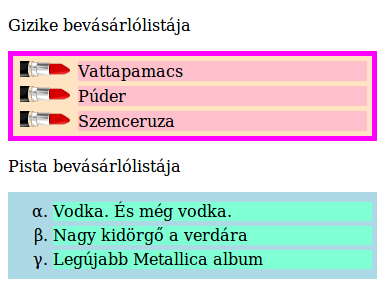
\includegraphics[width=\textwidth]{felsorolasok.png}
      \end{exampleblock}
  \end{columns} 
\end{frame}

\subsection{Táblázatok}

%_
\begin{frame}
  \begin{columns}[c]
    \column{0.5\textwidth}
      Táblázatok alapértelmezett formázása:
      \begin{itemize}
        \item Cellaméretek a tartalomhoz igazodnak
        \item Nincsenek szegélyek
        \item Fejléc (\texttt{<th>}) cellák félkövérek, középre zártak
        \item Normál cellák (\texttt{<td>}) balra zártak
      \end{itemize}
    \column{0.45\textwidth}
        \begin{exampleblock}{\textattachfile{tablazat01.html}{tablazat01.html}}
          \begin{center}
            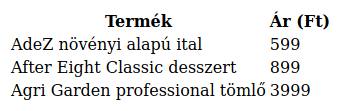
\includegraphics[width=\textwidth]{tablazat01.png}
          \end{center}
        \end{exampleblock}
  \end{columns}
\end{frame}

%_
\begin{frame}
  Kaphat szegélyt a teljes táblázat \dots
  \begin{columns}[c]
    \column{0.66\textwidth}
      \begin{exampleblock}{\textattachfile{tablazat02.html}{tablazat02.html}}
        \scriptsize
        \lstinputlisting[style=HTML,linerange={7-7},numbers=left,firstnumber=7]{tablazat02.html}
        \lstinputlisting[style=HTML,linerange={11-16},numbers=left,firstnumber=11]{tablazat02.html}
      \end{exampleblock}
    \column{0.3\textwidth}
      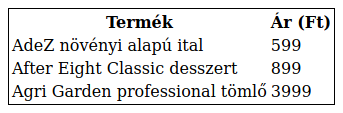
\includegraphics[width=\textwidth]{tablazat02.png}
  \end{columns}
\end{frame}

%_
\begin{frame}
  \dots vagy annak cellái \dots
  \vfill
  \begin{exampleblock}{\textattachfile{tablazat03.html}{tablazat03.html}}
    \lstinputlisting[style=HTML,linerange={7-7},numbers=left,firstnumber=7]{tablazat03.html}
  \end{exampleblock}
  \begin{center}
    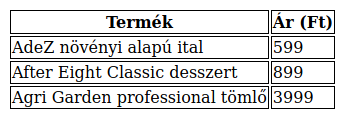
\includegraphics[width=0.4\textwidth]{tablazat03.png}
  \end{center}
\end{frame}

%_
\begin{frame}
  \dots vagy mindkettő.
  \vfill
  \begin{exampleblock}{\textattachfile{tablazat04.html}{tablazat04.html}}
    \lstinputlisting[style=HTML,linerange={7-7},numbers=left,firstnumber=7]{tablazat04.html}
  \end{exampleblock}
  \begin{center}
    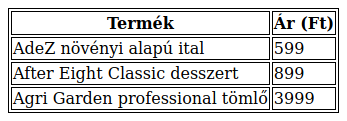
\includegraphics[width=0.4\textwidth]{tablazat04.png}
  \end{center}
\end{frame}

%_
\begin{frame}
  A cellák közötti távolság változtatható a \texttt{<table>} \texttt{border-spacing} tulajdonságával \dots
  \vfill
  \begin{exampleblock}{\textattachfile{tablazat05.html}{tablazat05.html}}
    \lstinputlisting[style=HTML,linerange={7-8},numbers=left,firstnumber=7]{tablazat05.html}
  \end{exampleblock}
  \begin{center}
    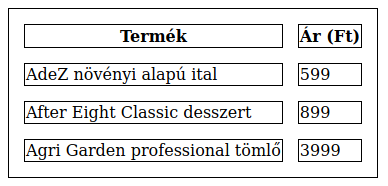
\includegraphics[width=0.4\textwidth]{tablazat05.png}
  \end{center}
\end{frame}

%_
\begin{frame}
  \dots de teljesen el is tüntethető a \texttt{<table>} \texttt{border-collapse} tulajdonságával:
  \begin{description}[m]
    \item[\texttt{separate}] elkülönített cellák, alapértelmezés.
    \item[\texttt{collapse}] összevont cellaszegélyek.
  \end{description}
  \vfill
  \begin{exampleblock}{\textattachfile{tablazat06.html}{tablazat06.html}}
    \lstinputlisting[style=HTML,linerange={7-8},numbers=left,firstnumber=7]{tablazat06.html}
  \end{exampleblock}
  \begin{center}
    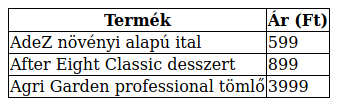
\includegraphics[width=0.4\textwidth]{tablazat06.png}
  \end{center}
\end{frame}

%_
\begin{frame}
  A cellák szegélye és tartalma közötti távolság a \texttt{<td>}, \texttt{<th>} \texttt{padding} tulajdonságával állítható.
  \begin{exampleblock}{\textattachfile{tablazat07.html}{tablazat07.html}}
    \footnotesize
    \lstinputlisting[style=HTML,linerange={7-11},numbers=left,firstnumber=7]{tablazat07.html}
  \end{exampleblock}
  \begin{center}
    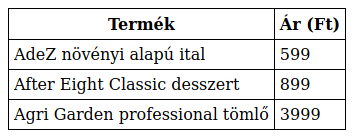
\includegraphics[width=0.4\textwidth]{tablazat07.png}
  \end{center}
\end{frame}

%_
\begin{frame}
  A cellákon belüli igazítás a \texttt{text-align}, \texttt{vertical-align} tulajdonságokkal állítható.
  \begin{exampleblock}{\textattachfile{tablazat08.html}{tablazat08.html}}
    \scriptsize
    \lstinputlisting[style=HTML,linerange={7-13},numbers=left,firstnumber=7]{tablazat08.html}
  \end{exampleblock}
  \begin{center}
    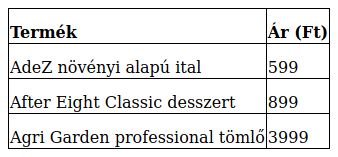
\includegraphics[width=0.35\textwidth]{tablazat08.png}
  \end{center}
\end{frame}

%_
\begin{frame}
  Ha a táblázat szélesebb, mint amit a tartalom indokol, a maradék hely arányosan lesz elosztva.
  \begin{exampleblock}{\textattachfile{tablazat09.html}{tablazat09.html}}
    \scriptsize
    \lstinputlisting[style=HTML,linerange={7-14},numbers=left,firstnumber=7]{tablazat09.html}
  \end{exampleblock}
  \begin{center}
    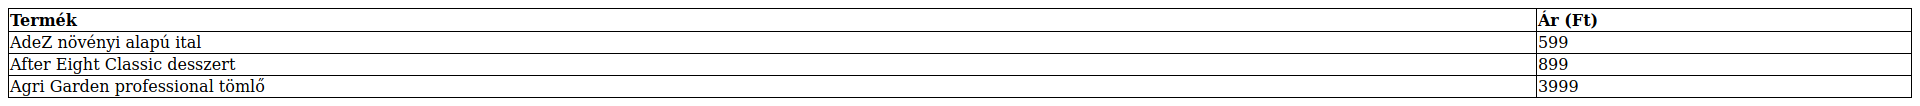
\includegraphics[width=\textwidth]{tablazat09.png}
  \end{center}
\end{frame}

%_
\begin{frame}
  \begin{columns}[c]
    \column{0.3\textwidth}
      \small
      Az olvashatóság javításához pl. kiemelhetjük az egér alatti sort a \texttt{:hover} látszólagos osztállyal.\\
      Figyeljük meg a ,,csíkozást''!
      \vfill
      \begin{center}
        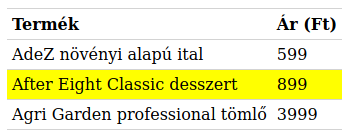
\includegraphics[width=\textwidth]{tablazat10.png}
      \end{center}
    \column{0.66\textwidth}
      \begin{exampleblock}{\textattachfile{tablazat10.html}{tablazat10.html}}
        \scriptsize
        \lstinputlisting[style=HTML,linerange={7-14},numbers=right,firstnumber=7]{tablazat10.html}
      \end{exampleblock}
  \end{columns}
\end{frame}

%_
\begin{frame}
  Az olvashatóság a sorok váltakozó háttérszínével is javítható. Egy szülő elem (pl. \texttt{<table>}) gyerekei (sorok) közül meghatározottak kiválasztása: \hiv{\href{https://developer.mozilla.org/en-US/docs/Web/CSS/:nth-child}{\texttt{nth-child()}}} látszólagos osztállyal.
  \begin{columns}[c]
    \column{0.66\textwidth}
      \begin{description}[m]
        \item[\texttt{An+b}] \hfill \\ $n = 0 \dots$, de a gyerekek számozása 1-től indul!
        \item[\texttt{even}] \hfill \\ Páros elemek $\equiv$ \texttt{2n}
        \item[\texttt{odd}] \hfill \\ Páratlan elemek $\equiv$ \texttt{2n+1}
      \end{description}
    \column{0.3\textwidth}
      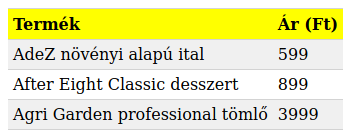
\includegraphics[width=\textwidth]{tablazat11.png}
  \end{columns} 
\end{frame}

%_
\begin{frame}
  \begin{exampleblock}{\textattachfile{tablazat11.html}{tablazat11.html}}
    \small
    \lstinputlisting[style=HTML,linerange={7-17},numbers=left,firstnumber=7]{tablazat11.html}
  \end{exampleblock}
\end{frame}

%_
\begin{frame}
  \begin{columns}[c]
    \column{0.66\textwidth}
      Görgethető táblázat, trükkök:
      \begin{itemize}
        \item Rögzített fejléc $\to$ két külön táblázat, csak az alsó görgethető
        \item Görgetés: táblázat beágyazva egy túl alacsony elembe, és \texttt{overflow-y: scroll} (hasonlóan a vízszintes irányú görgetés is lehetséges az \texttt{overflow-x} tulajdonsággal)
        \item Legyenek a két táblázat oszlopai rendre azonos szélességűek!
      \end{itemize}
    \column{0.3\textwidth}
      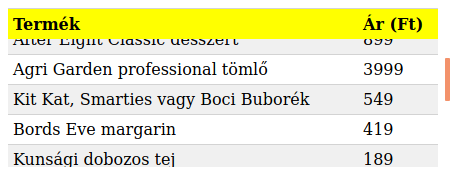
\includegraphics[width=\textwidth]{tablazat12.png}
  \end{columns}
\end{frame}

%_
\begin{frame}
  \begin{exampleblock}{\textattachfile{tablazat12.html}{tablazat12.html}}
    \fontsize{7}{8} \selectfont
    \lstinputlisting[style=HTML,linerange={28-41},numbers=left,firstnumber=28]{tablazat12.html}
    \lstinputlisting[style=HTML,linerange={51-53},numbers=left,firstnumber=51]{tablazat12.html}
  \end{exampleblock}
\end{frame}

%_
\begin{frame}
  \begin{exampleblock}{\textattachfile{tablazat12.html}{tablazat12.html}}
    \fontsize{7}{8} \selectfont
    \lstinputlisting[style=HTML,linerange={7-24},numbers=left,firstnumber=7]{tablazat12.html}
  \end{exampleblock}
\end{frame}

%_
\begin{frame}
  Táblázat címkéjének elhelyezése: \texttt{caption-side}
  \begin{description}[m]
    \item[\texttt{top}] \hfill \\ Fent, alapértelmezés.
    \item[\texttt{bottom}] \hfill \\ Lent.
  \end{description}
  \vfill
  Üres cellák szegélyeinek rajzolása: \texttt{empty-cells}
  \begin{description}[m]
    \item[\texttt{show}] \hfill \\ Megrajzolja, alapértelmezés.
    \item[\texttt{hide}] \hfill \\ Nem rajzolja meg.
  \end{description}
\end{frame}

%_
\begin{frame}
  Táblázat megjelenítési algoritmus: \texttt{table-layout}
  \begin{description}[m]
    \item[\texttt{auto}] \hfill \\ A cellák szélessége a legszélesebb nem tördelhető tartalmi elem függvénye. Alapértelmezés.
    \item[\texttt{fixed}] \hfill \\ Az oszlopok szélességét vagy
    \begin{itemize}
      \item a \texttt{<table>} és \texttt{<col>} elemek szélességei adják meg, vagy
      \item az első sor celláinak szélességei. Ha ilyen nincs, egyforma szélesek lesznek a cellák.
    \end{itemize}
    Nagy táblázatoknál jelentősen gyorsabb megjelenés.
  \end{description}
\end{frame}

%_
\begin{frame}
  Készítse el a \textattachfile{queen.png}{queen.png} fájl felhasználásával az alábbi weboldalt, ami a \hiv{\href{https://hu.wikipedia.org/wiki/Nyolckir\%C3\%A1lyn\%C5\%91-probl\%C3\%A9ma}{Nyolckirálynő probléma}} egy lehetséges megoldását mutatja! Ügyeljen rá, hogy keskeny kijelzőkön a táblázat vízszintesen görgethető legyen! (A cellák 50x50, a képek 40x40px méretűek.)
  \begin{exampleblock}{\textattachfile{sakk.html}{sakk.html}}
    \begin{center}
      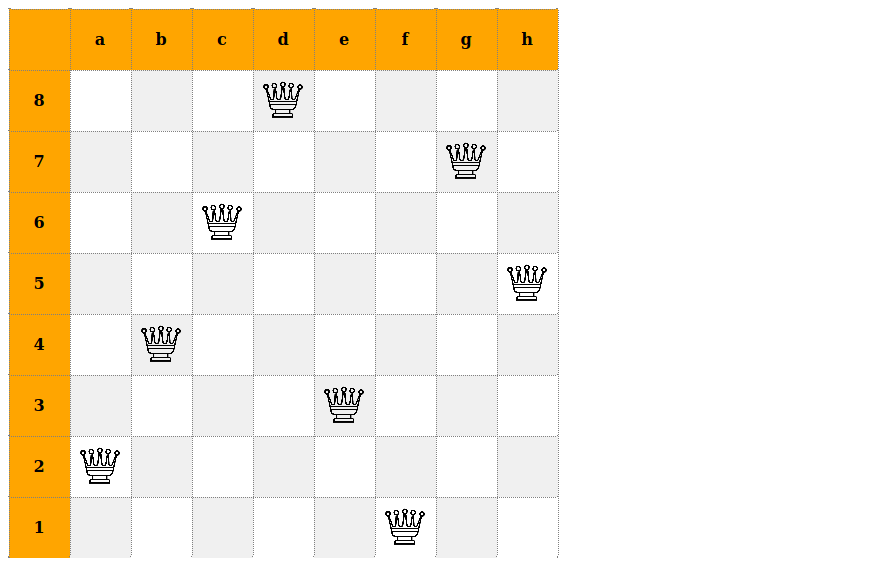
\includegraphics[scale=0.15]{sakk1.png}\hspace{1cm}
      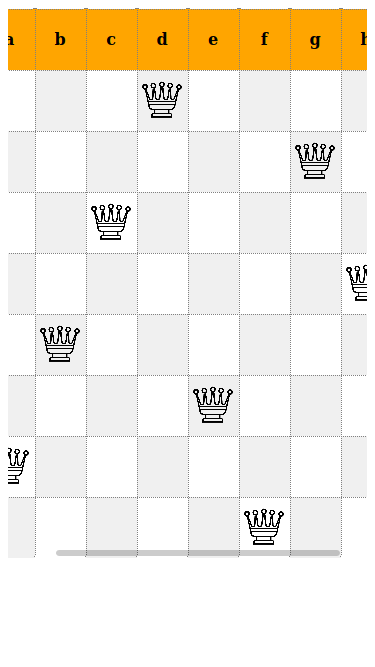
\includegraphics[scale=0.15]{sakk2.png}
    \end{center}
  \end{exampleblock}  
\end{frame}

\subsection{Megjelenítés}

%_
\begin{frame}
  A \texttt{display} tulajdonsággal állítható egy elem \emph{megjelenése}:
  \begin{description}[m]
    \item[\texttt{block}] \hfill \\ Blokkszintű megjelenítés
    \item[\texttt{inline}] \hfill \\ Soron belüli megjelenítés
    \item[\texttt{none}] \hfill \\ Nincs megjelenítés
  \end{description}
\end{frame}

%_
\begin{frame}
  \begin{description}[m]
    \item[Blokkszintű elemek] \hfill \\ Pl. \texttt{<p>}, \texttt{<div>}. Új sorban kezdődik, vízszintesen elfoglalja a teljes rendelkezésre álló helyet.
    \item[Soron belüli elemek] \hfill \\ Pl. \texttt{<a>}, \texttt{<span>}. Sor (blokk) belsejében kezdődik, annyi helyet foglal, amennyit a tartalom kíván.
  \end{description}
  \vfill
  JavaScript programok gyakran használják a \texttt{none} értéket bizonyos tartalmak ideiglenes elrejtésére/megjelenítésére a DOM módosítása helyett.
\end{frame}

%_
\begin{frame}
  \begin{columns}[c]
    \column{0.66\textwidth}
      A \texttt{visibility} tulajdonsággal állítható egy elem \emph{láthatósága}:
      \begin{description}[m]
        \item[\texttt{visible}] \hfill \\ Látható.
        \item[\texttt{hidden}] \hfill \\ Rejtett, de az elhelyezéséhez szükséges helyet a böngésző fenntartja!
      \end{description}
    \column{0.3\textwidth}
      \begin{exampleblock}{\textattachfile{display.html}{display.html}}
        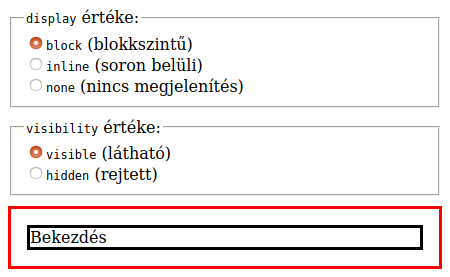
\includegraphics[width=\textwidth]{display.png}
      \end{exampleblock}
  \end{columns}
  
\end{frame}

\subsection{Elemek elhelyezése}

%_
\begin{frame}
  \begin{columns}[c]
    \column{0.5\textwidth}
      A \texttt{position} tulajdonsággal befolyásolható az elemek elhelyezési módja az oldalon. Értékei:
      \begin{description}[m]
        \item[\texttt{static}] \hfill \\ Alapértelmezett elrendezés. A böngésző dönt az elemek helyéről és ált. a méretezéséről is (pl. blokkszintű elemek egymás alatt/egymáson belül, széltében kitöltik a rendelkezésre álló helyet, soron belüliek a blokkszintűek belsejében, stb.)
      \end{description}
    \column{0.45\textwidth}
      \begin{exampleblock}{\textattachfile{static.html}{static.html}}
        \scriptsize
        \lstinputlisting[style=HTML,linerange={7-12},numbers=right,firstnumber=7]{static.html}
        \lstinputlisting[style=HTML,linerange={16-18},numbers=right,firstnumber=16]{static.html}
      \end{exampleblock}
      \begin{center}
        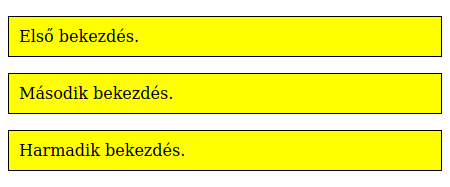
\includegraphics[width=0.5\textwidth]{static.png}
      \end{center}
  \end{columns}
\end{frame}

%_
\begin{frame}
  \begin{columns}[T]
    \column{0.35\textwidth}
      \begin{description}[m]
        \item[\texttt{relative}] \hfill \\ Az elem az eredeti helyéhez képest eltolható, de ezt a régi helyet a böngésző fenntartja. Megadható az elem tetejének (\texttt{top}), aljának (\texttt{bottom}), bal (\texttt{left}) és jobb oldalának (\texttt{right}) relatív helyzete.
      \end{description}
      \vfill
      \begin{center}
        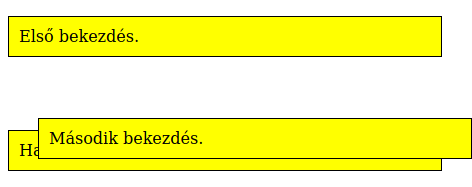
\includegraphics[width=.75\textwidth]{relative.png}
      \end{center}
    \column{0.6\textwidth}
      \begin{exampleblock}{\textattachfile{relative.html}{relative.html}}
        \scriptsize
        \lstinputlisting[style=HTML,linerange={7-16},numbers=right,firstnumber=7]{relative.html}
        \lstinputlisting[style=HTML,linerange={20-22},numbers=right,firstnumber=20]{relative.html}
      \end{exampleblock}
  \end{columns}
\end{frame}

%_
\begin{frame}
  \begin{description}[m]
    \item[\texttt{absolute}] \hfill \\ A legközelebbi, nem statikusan elhelyezett szülő elemhez, annak hiányában a dokumentum testéhez képest relatívan megadott helyre igazítja az elemet. Az elem eredeti helyét nem őrzi meg a böngésző.
  \end{description}
  \vfill
  \begin{center}
    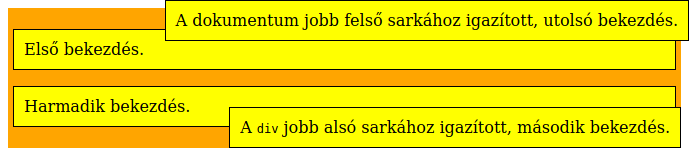
\includegraphics[width=.6\textwidth]{absolute.png}\\
    \textattachfile{absolute.html}{absolute.html}
  \end{center}
\end{frame}

%_
\begin{frame}
  \begin{columns}[c]
    \column{0.45\textwidth}
      \begin{exampleblock}{\textattachfile{absolute.html}{absolute.html}}
        \fontsize{7}{8} \selectfont
        \lstinputlisting[style=HTML,linerange={7-22},numbers=left,firstnumber=7]{absolute.html}
      \end{exampleblock}
    \column{0.5\textwidth}
      \begin{exampleblock}{}
        \fontsize{7}{8} \selectfont
        \lstinputlisting[style=HTML,linerange={23-28},numbers=right,firstnumber=23]{absolute.html}
        \lstinputlisting[style=HTML,linerange={32-41},numbers=right,firstnumber=32]{absolute.html}
      \end{exampleblock}
  \end{columns}
\end{frame}

%_
\begin{frame}
  \begin{description}[m]
    \item[\texttt{fixed}] \hfill \\ Az elem pozíciója a nézetablakhoz képest relatív, görgetés közben is a helyén marad.
  \end{description}
  \begin{columns}[c]
    \column{0.45\textwidth}
      \begin{center}
        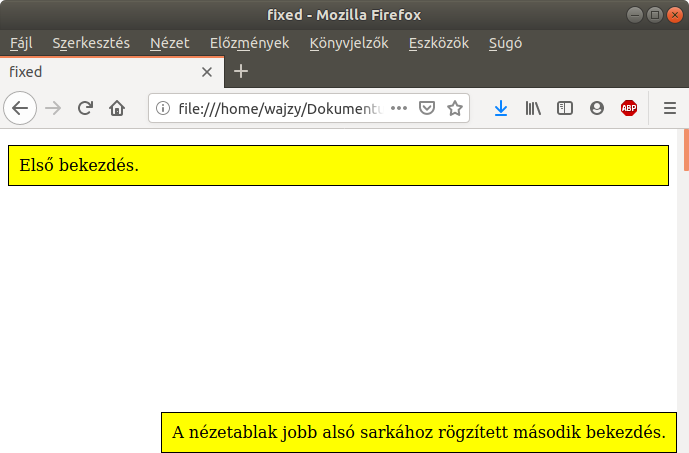
\includegraphics[width=\textwidth]{fixed1.png}
      \end{center}
    \column{0.45\textwidth}
      \begin{center}
        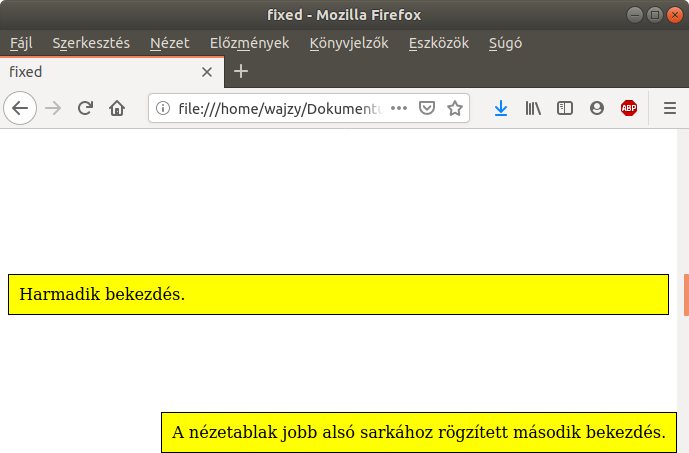
\includegraphics[width=\textwidth]{fixed2.png}
      \end{center}
  \end{columns}
  \begin{center}
    \textattachfile{fixed.html}{fixed.html} -- Figyeljék a gördítősávot!
  \end{center}
\end{frame}

%_
\begin{frame}
  \begin{columns}[T]
    \column{0.43\textwidth}
      \begin{exampleblock}{\textattachfile{fixed.html}{fixed.html}}
        \scriptsize
        \lstinputlisting[style=HTML,linerange={7-18},numbers=left,firstnumber=7]{fixed.html}
      \end{exampleblock}
    \column{0.53\textwidth}
      \begin{exampleblock}{}
        \scriptsize
        \lstinputlisting[style=HTML,linerange={22-26},numbers=right,firstnumber=22]{fixed.html}
      \end{exampleblock}
  \end{columns}  
\end{frame}

%_
\begin{frame}
  \begin{description}[m]
    \item[\texttt{sticky}] \hfill \\ A \texttt{relative} és a \texttt{fixed} kombinációja; az elem gördül a nézetablak tartalmával, amíg el nem ér egy adott helyre, ahová ,,odaragad''.\\
    \vspace{0.3cm} \tiny Részleges böngésző támogatás; pl. Safarin a \texttt{-webkit-sticky} értékkel működik csak.
  \end{description}
  \begin{columns}[T]
    \column{0.3\textwidth}
      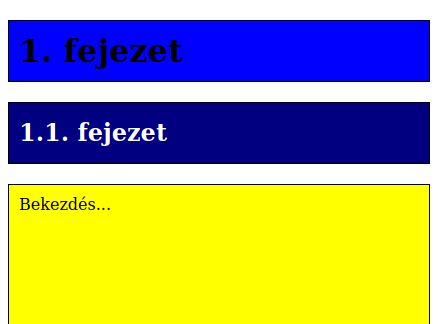
\includegraphics[width=\textwidth]{sticky1.png}
    \column{0.3\textwidth}
      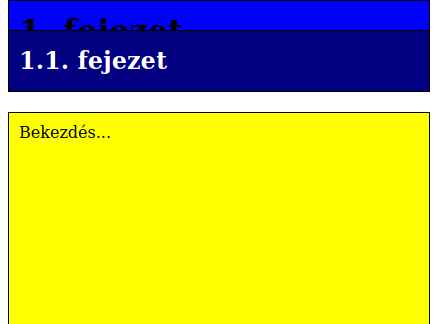
\includegraphics[width=\textwidth]{sticky2.png}
    \column{0.3\textwidth}
      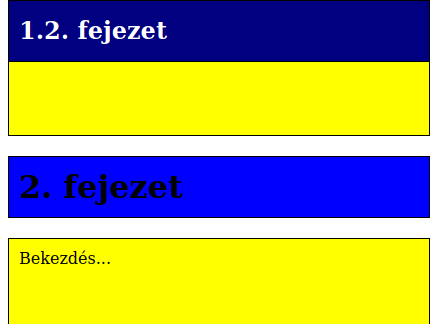
\includegraphics[width=\textwidth]{sticky3.png}
  \end{columns}
  \begin{center}
    \textattachfile{sticky.html}{sticky.html} -- Próbálják görgetni a tartalmat!
  \end{center}
\end{frame}

%_
\begin{frame}
  \begin{columns}[c]
    \column{0.45\textwidth}
      \begin{exampleblock}{\textattachfile{sticky.html}{sticky.html}}
        \fontsize{7}{8} \selectfont
        \lstinputlisting[style=HTML,linerange={7-23},numbers=left,firstnumber=7]{sticky.html}
      \end{exampleblock}
    \column{0.5\textwidth}
      \begin{exampleblock}{}
        \fontsize{7}{8} \selectfont
        \lstinputlisting[style=HTML,linerange={24-29},numbers=right,firstnumber=24]{sticky.html}
        \lstinputlisting[style=HTML,linerange={33-39},numbers=right,firstnumber=33]{sticky.html}
      \end{exampleblock}
  \end{columns}
\end{frame}

%_
\begin{frame}
  Próbálja meg elkészíteni az alábbi \textattachfile{gabor.html}{weboldalt} a \textattachfile{gabor.txt}{gabor.txt} és \textattachfile{gabor.jpeg}{gabor.jpeg} fájlok felhasználásával!
  \vfill
  \begin{columns}[T]
    \column{0.3\textwidth}
      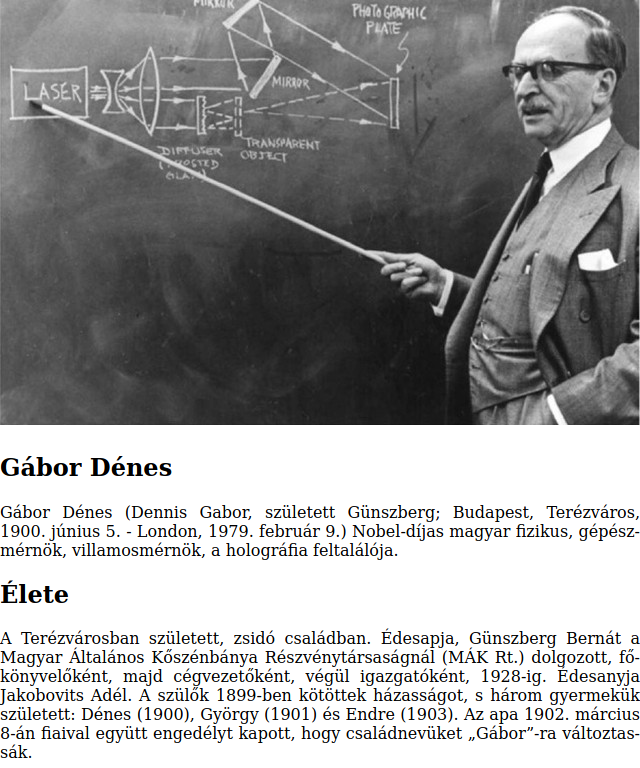
\includegraphics[width=\textwidth]{gabor1.png}
    \column{0.3\textwidth}
      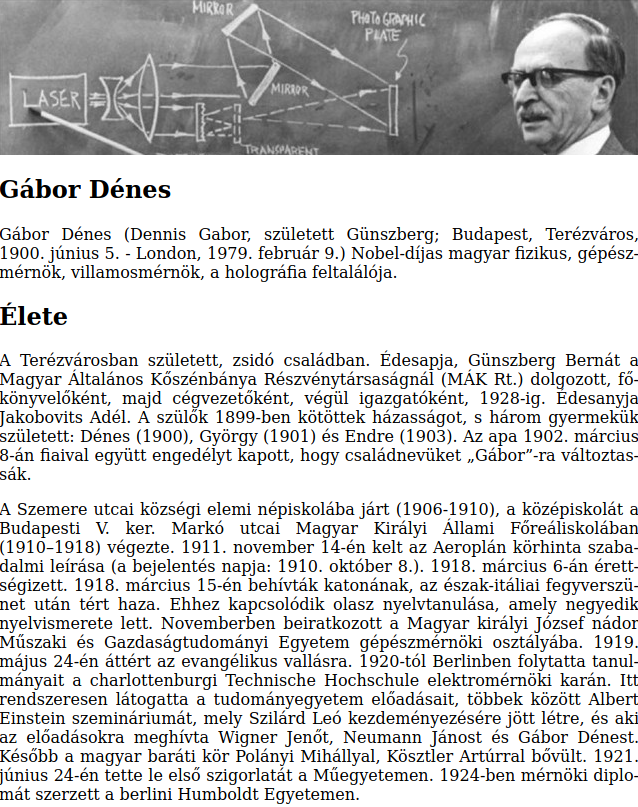
\includegraphics[width=\textwidth]{gabor2.png}
    \column{0.3\textwidth}
      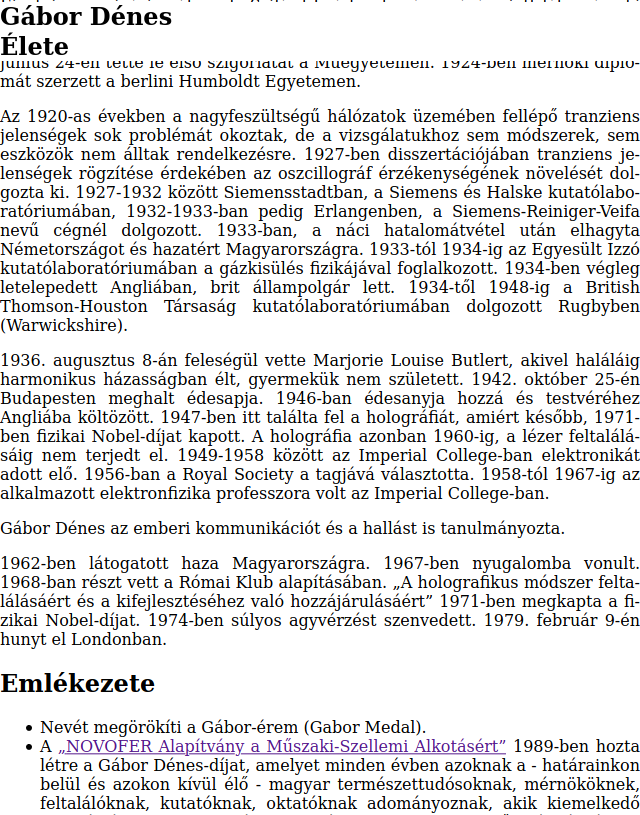
\includegraphics[width=\textwidth]{gabor3.png}
  \end{columns}
\end{frame}

%_
\begin{frame}
  Az oldal elvárt viselkedése a következő:
  \begin{itemize}
    \item A kép egyhelyben áll a görgetés hatására is. A felfelé gördülő szöveg lassan rácsúszik, majd teljesen kitakarja azt.
    \item Az első szintű címsor addig csúszik felfelé, amíg el nem éri a nézetablak tetejét. Utána ottmarad, és a bekezdések szövege alágördül.
    \item A második szintű címsor hasonlóan viselkedik az első szintűhöz, de az alatt áll meg, nem takarja le azt. A második szintű címsorok viszont letakarhatják egymást.
    \item A cikk maximális szélessége 640 képpont. Ha ennél több hely áll rendelkezésre, középre kell igazítani.
    \item A szöveg sorkizárt igazítású, automatikusan elválasztott.
    \item Az idézetek előtt és után magyar stílusú (,, '') idézőjeleket alkalmaz.
    \item A hivatkozás új oldalon nyílik meg.
  \end{itemize}
\end{frame}

\subsection{Számlálók}

%_
\begin{frame}
  Számlálók: mint egy program változói, melyek értéke változik (ált. nő) a használat hatására\\
  Használható pl. fejezetek vagy felsorolások számozására
  \vfill
  \texttt{counter-reset}: számláló létrehozása, újraindítása vagy kezdőértékkel ellátása.
  \begin{description}[m]
    \item[\texttt{none}] \hfill \\ Számlálók nem lesznek inicializálva, alapértelmezés.
    \item[\texttt{id number}] \hfill \\ Az \emph{id} azonosítójú számláló felveszi a \emph{number} értéket. Utóbbi elhagyható, alapértelmezetten 0.
  \end{description}
\end{frame}

%_
\begin{frame}
  \texttt{counter-increment}: számláló értékének léptetése
  \begin{description}[m]
    \item[\texttt{none}] \hfill \\ Nem változtat a számlálók értékén, alapértelmezés.
    \item[\texttt{id number}] \hfill \\ Hozzáad \emph{number}-t (alapértelmezetten 1, de lehet akár negatív érték is) az \emph{id} számláló értékéhez. 
  \end{description}
  \vfill
  A \texttt{content} tulajdonságot használják a számlálók értékének kijelzésére, jellemzően a \texttt{::before} látszóleges elemben (\hiv{\href{https://developer.mozilla.org/en-US/docs/Web/CSS/::marker}{\texttt{::marker}}} gyengén támogatott). Ugyanitt ált. számláló növelésre is sor kerül.
\end{frame}

%_
\begin{frame}
  \texttt{counter(id)} vagy \texttt{counter(id, style)}: számláló értékének lekérdezése
  \begin{description}[m]
    \item[\texttt{id}] \hfill \\ A \texttt{counter-reset}-tel létrehozott és \texttt{counter-increment}-tel léptetett változó azonosítója.
    \item[\texttt{style}] \hfill \\ A számláló megjelenítési módja, pl. \texttt{lower-alpha}, \texttt{upper-roman}, \texttt{decimal-leading-zero}, stb., vagy a \hiv{\href{https://developer.mozilla.org/en-US/docs/Web/CSS/symbols}{\texttt{symbols()}}} függvénnyel adott szimbólumok.
  \end{description}
\end{frame}

%_
\begin{frame}
  \begin{columns}[c]
    \column{0.5\textwidth}
      \begin{exampleblock}{\textattachfile{szamozottFejezet.html}{szamozottFejezet.html}}
        \scriptsize
        \lstinputlisting[style=HTML,linerange={7-16},numbers=left,firstnumber=7]{szamozottFejezet.html}
      \end{exampleblock}
    \column{0.5\textwidth}
      \begin{exampleblock}{}
        \scriptsize
        \lstinputlisting[style=HTML,linerange={19-28},numbers=right,firstnumber=19]{szamozottFejezet.html}
      \end{exampleblock}
  \end{columns}
\end{frame}

%_
\begin{frame}
  \begin{center}
    
\includegraphics[width=.5\textwidth]{szamozottFejezet.png}\\
    \textattachfile{szamozottFejezet.html}{szamozottFejezet.html}
  \end{center}
\end{frame}

%_
\begin{frame}
  Egymásba ágyazott azonos típusú elemeknél (pl. \texttt{<ol>}, \texttt{<ul>}) rekurzívan mindig új számláló keletkezik. Megjelenítésük: \texttt{counters(id, string)} vagy \texttt{counters(id, string, style)} függvénnyel.
  \begin{description}[m]
    \item[\texttt{id}] \hfill \\ A számláló neve.
    \item[\texttt{string}] \hfill \\ A számlálók értékeit elválasztó karakterlánc.
    \item[\texttt{style}] \hfill \\ A számlálók stílusa.
  \end{description}
\end{frame}

%_
\begin{frame}
  \begin{columns}[c]
    \column{0.54\textwidth}
      \begin{exampleblock}{\textattachfile{szamozottLista.html}{szamozottLista.html}}
        \scriptsize
        \lstinputlisting[style=HTML,linerange={7-16},numbers=left,firstnumber=7]{szamozottLista.html}
      \end{exampleblock}
    \column{0.43\textwidth}
      \begin{exampleblock}{}
        \scriptsize
        \lstinputlisting[style=HTML,linerange={21-31},numbers=right,firstnumber=21]{szamozottLista.html}
      \end{exampleblock}
  \end{columns}
\end{frame}

%_
\begin{frame}
  \begin{center}
    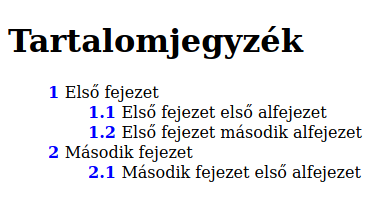
\includegraphics[width=.5\textwidth]{szamozottLista.png}\\
    \textattachfile{szamozottLista.html}{szamozottLista.html}
  \end{center}
\end{frame}

%_
\begin{frame}
  \begin{columns}[c]
    \column{0.8\textwidth}
      Készítse el a mellékelt \textattachfile{teendok.html}{teendok.html} oldalt!
      \begin{itemize}
        \item A kétszintű felsorolás külső szintjén alkalmazzon nagybetűs római számokat, a belsőn arab számokat!
        \item Utóbbiak számozása az egész oldalon legyen folytonos (1-6)!
        \item A számokat helyezze sárga hátterű ellipszisek közepébe, kék színnel és félkövér betűkkel megjelenítve!
      \end{itemize}
    \column{0.15\textwidth}
      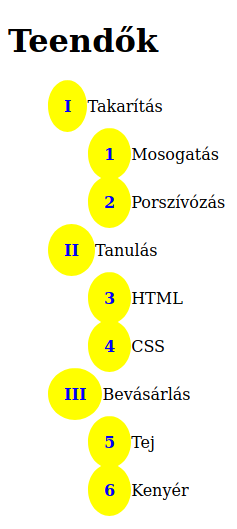
\includegraphics[width=\textwidth]{teendok.png}
  \end{columns}
\end{frame}

\subsection{Lebegtetés}

%_
\begin{frame}
  A \emph{lebegtetés} egy speciális oldalelrendezési módszer, amivel egy elemet a tárolóján belül mozgathatunk.
  A \texttt{float} tulajdonsággal állítható a lebegtetés iránya:
  \begin{description}[m]
    \item[\texttt{left}] \hfill \\ A tároló bal széle felé mozdítja az elemet. Ha nincs ott elég hely, egy ,,sorral'' lejjebb helyezi el.
    \item[\texttt{right}] \hfill \\ Jobb oldalra mozgat.
    \item[\texttt{none}] \hfill \\ Nincs lebegtetés, alapértelmezés.
  \end{description}
  Legegyszerűbb és jellemző felhasználás: kép körbefolyatása szöveggel. Hibalehetőség: a lebegtetett elem túlnyúlhat a tárolón.
\end{frame}

%_
\begin{frame}
  \begin{columns}[c]
    \column{0.45\textwidth}
      \begin{exampleblock}{\textattachfile{lebeg1.html}{lebeg1.html}}
        \scriptsize
        \lstinputlisting[style=HTML,linerange={7-15},numbers=left,firstnumber=7]{lebeg1.html}
      \end{exampleblock}
    \column{0.45\textwidth}
      \begin{exampleblock}{}
        \scriptsize
        \lstinputlisting[style=HTML,linerange={16-28},numbers=right,firstnumber=16]{lebeg1.html}
      \end{exampleblock}
  \end{columns}
\end{frame}

%_
\begin{frame}
  \begin{columns}[c]
    \column{0.66\textwidth}
      \begin{exampleblock}{\textattachfile{lebeg1.html}{lebeg1.html}}
        \fontsize{7}{8} \selectfont
        \lstinputlisting[style=HTML,linerange={32-35},numbers=left,firstnumber=32]{lebeg1.html}
        \lstinputlisting[style=HTML,linerange={48-52},numbers=left,firstnumber=48]{lebeg1.html}
      \end{exampleblock}
    \column{0.3\textwidth}
      \begin{exampleblock}{}
        \includegraphics[width=\textwidth]{lebeg1.png}
      \end{exampleblock}
  \end{columns}
\end{frame}

%_
\begin{frame}
  Gyakran használják a lebegtetést az oldalelrendezés kialakítására, pl. tartalmak helytől függően egymás mellé vagy alá igazításához.
  \vfill
  \begin{center}
    \includegraphics[width=\textwidth]{lebeg21.png}\\
    \textattachfile{lebeg2.html}{lebeg2.html}
  \end{center}
\end{frame}

%_
\begin{frame}
  \begin{columns}[c]
    \column{0.41\textwidth}
      \begin{exampleblock}{\textattachfile{lebeg2.html}{lebeg2.html}}
        \scriptsize
        \lstinputlisting[style=HTML,linerange={7-16},numbers=left,firstnumber=7]{lebeg2.html}
      \end{exampleblock}
    \column{0.54\textwidth}
      \begin{exampleblock}{}
        \scriptsize
        \lstinputlisting[style=HTML,linerange={20-28},numbers=right,firstnumber=20]{lebeg2.html}
      \end{exampleblock}
  \end{columns}
\end{frame}

%_
\begin{frame}
  Az oldalt lekicsinyítve viszont ismét kellemetlen mellékhatás lép fel:
  \vfill
  \begin{center}
    \includegraphics[width=.3\textwidth]{lebeg22.png}\\
    \textattachfile{lebeg2.html}{lebeg2.html}
  \end{center}
  Hogyan lehet úrrá lenni a gondokon?
\end{frame}

%_
\begin{frame}
  1. lehetőség: az \texttt{overflow} tulajdonság használata, de néha nem kívánt görgetősáv jelenik meg.
  \vfill
  \begin{columns}[c]
    \column{0.6\textwidth}
      \begin{exampleblock}{\textattachfile{lebeg3.html}{lebeg3.html}}
        \scriptsize
        \lstinputlisting[style=HTML,linerange={29-29},numbers=left,firstnumber=29]{lebeg3.html}
        \lstinputlisting[style=HTML,linerange={34-35},numbers=left,firstnumber=34]{lebeg3.html}
      \end{exampleblock}
    \column{0.35\textwidth}
      \includegraphics[width=\textwidth]{lebeg3.png}
  \end{columns}
\end{frame}

%_
\begin{frame}
  \begin{columns}[c]
    \column{0.7\textwidth}
      \footnotesize
      2. lehetőség: a \texttt{clear} tulajdonsággal megadható, hogy egy elem valamely oldalán nem szerepelhet lebegtetett elem.
      \begin{description}[m]
        \item[\texttt{none}] \hfill \\ Az elem mindkét oldalára kerülhet lebegtetett másik elem, alapértelmezés.
        \item[\texttt{left}] \hfill \\ Az elem bal oldalára nem kerülhet lebegtetett elem.
        \item[\texttt{right}] \hfill \\ Ugyanaz a jobb oldalon.
        \item[\texttt{both}] \hfill \\ Egyik oldalon sem lehet lebegtetett elem.
      \end{description}
      \begin{exampleblock}{}
        \scriptsize
        \lstinputlisting[style=HTML,linerange={17-17},numbers=left,firstnumber=17]{lebeg4.html}
      \end{exampleblock}
    \column{0.25\textwidth}
      \begin{exampleblock}{\textattachfile{lebeg4.html}{lebeg4.html}}
        \includegraphics[width=\textwidth]{lebeg4.png}
      \end{exampleblock}
  \end{columns}
\end{frame}

%_
\begin{frame}
  \begin{columns}[c]
    \column{0.66\textwidth}
      3. lehetőség: a \emph{clearfix hack} (széles körben alkalmazott)
      \begin{exampleblock}{\textattachfile{lebeg5.html}{lebeg5.html}}
        \scriptsize
        \lstinputlisting[style=HTML,linerange={29-33},numbers=left,firstnumber=29]{lebeg5.html}
        \lstinputlisting[style=HTML,linerange={38-39},numbers=left,firstnumber=38]{lebeg5.html}
      \end{exampleblock}
    \column{0.3\textwidth}
      \includegraphics[width=\textwidth]{lebeg5.png}
  \end{columns}
\end{frame}

%_
\begin{frame}
  \begin{columns}[T]
    \column{0.8\textwidth}
      \footnotesize
      Készítse el a Futókalandorok weboldalának \textattachfile{futokalandorok.html}{nyitóoldalát} az \hiv{\href{http://futokalandorok.hu/index.html}{eredeti oldal}} egyszerűsített változataként! (\textattachfile{futokalandorok.txt}{Nyers szöveg}.)
      \begin{itemize}
        \item Készítsen egy vízszintes elrendezésű menüt az oldal tetejére! Ha egy sorban nem férnek el a menüpontok, akkor azokat új sor(ok)ban kell elhelyezni.
        \item A menüsáv háttere halvány szürke.
        \item A ,,Futókalandorok'' főcím fekete, a menüpontok (most még sehová sem mutató) hivatkozásai középszürkék.
        \item Ha az egér a hivatkozás fölé kerül, színe feketére vált.
        \item A menü és a tartalmi rész között hagyjon ki egy kis helyet!
        \item A tartalmi rész két hasábos, melyek az oldal szélességének 50-50\%-át foglalják el. Hagyjon mindegyikben egy kis belső kitöltést!
        \item A bal hasábban jelenítse meg a \textattachfile{futokalandorok.svg}{logót}!
        \item A jobb hasáb utolsó bekezdését igazítsa jobbra!
      \end{itemize}
    \column{0.15\textwidth}
      \includegraphics[width=\textwidth]{futokalandorok2.png}
  \end{columns}
\end{frame}

%_
\begin{frame}
  \begin{center}
    \includegraphics[width=.75\textwidth]{futokalandorok1.png}\\
    \textattachfile{futokalandorok.html}{futokalandorok.html}
  \end{center}
\end{frame}

\subsection{Flexbox}

%
\begin{frame}
  \begin{columns}
    \column{0.45\textwidth}
      Oldalelrendezési módszer: az elemeket egy tároló belsejében jelenítik meg, egy (vagy több) tengely mentén felfűzve. A tároló (pl. \texttt{<div>} elem) \texttt{display} tulajdonságának értékei:
      \begin{description}[m]
        \item[\texttt{flex}] \hfill \\ Blokkszintű elemként
        \item[\texttt{inline-flex}] \hfill \\ Soron belüli elemként
      \end{description}
    \column{0.45\textwidth}
      \begin{exampleblock}{\textattachfile{flexbox.html}{flexbox.html}}
        \scriptsize
        \lstinputlisting[style=HTML,linerange={7-17},numbers=right,firstnumber=7]{flexbox.html}
      \end{exampleblock}
  \end{columns}
\end{frame}

%
\begin{frame}
  A tengely és bejárásának iránya a \texttt{flex-direction} tulajdonsággal változtatható:
  \begin{columns}
    \column{0.35\textwidth}
      \begin{description}[m]
        \item[\texttt{row}] \hfill \\ Vízszintes, balról jobbra (alapértelmezés)
        \item[\texttt{row-reverse}] \hfill \\ Vízszintes, jobbról balra
        \item[\texttt{column}] \hfill \\ Függőleges, fentről le
        \item[\texttt{column-reverse}] \hfill \\ Függőleges, lentről fel
      \end{description}
    \column{0.55\textwidth}
      \begin{exampleblock}{\textattachfile{flexbox.html}{flexbox.html}}
        \scriptsize
        \lstinputlisting[style=HTML,linerange={21-26},numbers=right,firstnumber=21]{flexbox.html}
      \end{exampleblock}
      \includegraphics[width=\textwidth]{flex-direction-row.png}
  \end{columns}
\end{frame}

%
\begin{frame}
  Ha az elemek szélességeinek összege kisebb, mint a tengely hossza, akkor a \texttt{justify-content} tulajdonsággal beállítható, hová helyezzük az elemeket a tengely mentén:
  \begin{description}[m]
    \item[\texttt{flex-start}] \hfill \\ Alapértelmezés, a tengely elejére
    \item[\texttt{flex-end}] \hfill \\ A tengely végére
    \item[\texttt{center}] \hfill \\ Tengely közepére
    \item[\texttt{space-between}] \hfill \\ A tárolt elemek között egyforma méretű helyet hagy
    \item[\texttt{space-around}] \hfill \\ Minden tárolt elem mindkét oldalán azonos helyet hagy, a szomszédos üres részeket nem vonja össze
  \end{description}
\end{frame}

%
\begin{frame}
  \begin{exampleblock}{\textattachfile{flexbox.html}{flexbox.html}}
    \scriptsize
    \lstinputlisting[style=HTML,linerange={57-68},numbers=left,firstnumber=57]{flexbox.html}
  \end{exampleblock}
\end{frame}

%
\begin{frame}
  \begin{center}
    \includegraphics[width=.75\textwidth]{justify-content-space-between.png}
  \end{center}
\end{frame}

%
\begin{frame}
  Ha az elemek nem férnek el egymás mellett a tengely mentén, akkor a \texttt{flex-wrap} tulajdonságtól függ, mi történik:
  \begin{description}[m]
    \item[\texttt{nowrap}] \hfill \\ Alapértelmezés, a tárolt elemek kilógnak / nem jelennek meg
    \item[\texttt{wrap}] \hfill \\ További párhuzamos tengelyeket hoz létre
    \item[\texttt{wrap-reverse}] \hfill \\ Mint \texttt{wrap}, de a tengelyek sorrendje fordított
  \end{description}
  \vfill
  A \texttt{flex-direction} és \texttt{flex-wrap} tulajdonságok egy összetett tulajdonságon keresztül is állíthatók: \\
  \texttt{flex-flow: \emph{flex-direction flex-wrap}}
\end{frame}

%
\begin{frame}
  \begin{exampleblock}{\textattachfile{flexbox.html}{flexbox.html}}
    \scriptsize
    \lstinputlisting[style=HTML,linerange={107-109},numbers=left,firstnumber=107]{flexbox.html}
    \lstinputlisting[style=HTML,linerange={116-117},numbers=left,firstnumber=116]{flexbox.html}
  \end{exampleblock}
  \begin{columns}
    \column{0.55\textwidth}
      \includegraphics[width=\textwidth]{flex-wrap1.png}
    \column{0.4\textwidth}
      \includegraphics[width=\textwidth]{flex-wrap2.png}
  \end{columns}
\end{frame}

%
\begin{frame}
  Az elemeknek a tengelyre merőleges irányban történő méretezését / elhelyezését befolyásolja az \texttt{align-items} tulajdonság:
  \begin{description}[m]
    \item[\texttt{stretch}] \hfill \\ Kinyújtás a tároló széléig
    \item[\texttt{flex-start}] \hfill \\ Az elemeket balra / felfelé igazítja
    \item[\texttt{flex-end}] \hfill \\ Jobbra / lefelé igazít
    \item[\texttt{center}] \hfill \\ Középre igazít
    \item[\texttt{baseline}] \hfill \\ Az alapvonalhoz igazít
  \end{description}
\end{frame}

%
\begin{frame}
  A tárolóra beállított \texttt{align-items} minden elem megjelenítését befolyásolja, de ez az elemek \texttt{align-self} tulajdonságán keresztül egyedileg felülírható.
  \vfill
  \begin{columns}
    \column{0.65\textwidth}
      \begin{exampleblock}{\textattachfile{flexbox.html}{flexbox.html}}
        \scriptsize
        \lstinputlisting[style=HTML,linerange={99-106},numbers=left,firstnumber=99]{flexbox.html}
      \end{exampleblock}
    \column{0.3\textwidth}
      \includegraphics[width=\textwidth]{align-self.png}
  \end{columns}
\end{frame}

%
\begin{frame}
  Az \texttt{align-content} a tengelyek tárolón belüli elhelyezését befolyásolja. Értékei ugyanazok, mint \texttt{align-items}-nek. Akkor látványos a hatása, ha több tengelyre van szükség az elemek elhelyezéséhez.
  \vfill
  Ha az elemek HTML-ben specifikált sorrendjétől eltérő sorrendben szeretnénk azokat a tengelyre felfűzni, minden elemhez megadhatjuk a kívánt pozíciót az \texttt{order} tulajdonság értékeként.
  \vfill
  \begin{columns}
    \column{0.65\textwidth}
      \begin{exampleblock}{\textattachfile{flexbox.html}{flexbox.html}}
        \scriptsize
        \lstinputlisting[style=HTML,linerange={151-156},numbers=left,firstnumber=151]{flexbox.html}
      \end{exampleblock}
    \column{0.3\textwidth}
      \includegraphics[width=\textwidth]{order.png}
  \end{columns}
\end{frame}

%
\begin{frame}
  Az elemek között arányosan szétosztható a konténer területe, azok \texttt{flex} tulajdonságainak beállításával: \texttt{flex: \emph{flex-grow flex-shrink flex-basis}}
  \vfill
  \begin{columns}
    \column{0.6\textwidth}
      \begin{exampleblock}{\textattachfile{flexbox.html}{flexbox.html}}
        \scriptsize
        \lstinputlisting[style=HTML,linerange={163-168},numbers=left,firstnumber=163]{flexbox.html}
      \end{exampleblock}
    \column{0.35\textwidth}
      \includegraphics[width=\textwidth]{flex.png}
  \end{columns}
  \vfill
  Beállítások hatása gyakorlatban kipróbálható: \textattachfile{flextest.html}{flextest.html}
\end{frame}

\subsection{Összefoglaló feladatok}


\newcounter{feladatSzamlalo}

%_
\begin{frame}
  Készítse el a \hiv{\href{https://hu.wikipedia.org/wiki/Cascading_Style_Sheets}{CSS wiki oldala}} által ihletett weblapot!
  \begin{columns}[c]
    \column{0.25\textwidth}
      \begin{exampleblock}{\textattachfile{css.html}{css.html}}
        \includegraphics[width=\textwidth]{css1.pdf}
      \end{exampleblock}
    \column{0.75\textwidth}
      \begin{enumerate}
        \scriptsize
        \item Induljon ki a \textattachfile{css.txt}{css.txt} fájlból!
        \item Készítsen ebből magyar nyelvű HTML5 dokumentumot, UTF-8 karakterkódolással!
        \item Az oldal első szintű címsora és a böngészőfülön megjelenő szöveg egyaránt legyen ,,Cascading Style Sheets''!
        \item Ezt válassza el egy vízszintes vonallal...
        \item ...a második szintű címsorként jelölt sortól (,,A Wikipédiából, \dots'')! A ,,Tartalomjegyzék'' és az ,,Áttekintés'' szintén 2. szintű címsorként legyen jelölve!
        \item Az első bekezdés elején álló ,,CSS''-t jelölje meg rövidítésként! Ha valaki fölötte tartja az egeret, jelenjen meg a ,,Cascading Style Sheets, magyarul: lépcsőzetes stíluslapok'' szöveg egy buborékban!
        \item Jelölje meg hivatkozásként a ,,HTML'' szót, ami a megfelelő Wikipédia oldalra mutat!
        \item Járjon el ugyanígy az ,,XHTML''-lel is, de azt új fülön nyissa meg!
        \setcounter{feladatSzamlalo}{\theenumi}
      \end{enumerate}
  \end{columns}
\end{frame}

%_
\begin{frame}
  \begin{columns}[c]
    \column{0.25\textwidth}
      \begin{exampleblock}{\textattachfile{css.html}{css.html}}
        \includegraphics[width=\textwidth]{css2.pdf}
      \end{exampleblock}
    \column{0.75\textwidth}
      \begin{enumerate}
        \footnotesize
        \setcounter{enumi}{\thefeladatSzamlalo}
        \item A dokumentum tartalma alkosson egy cikket!
        \item Minden, ami a tartalomjegyzék felett van, legyen fejlécként jelölve!
        \item Külön szakaszként jelölje a tartalomjegyzéket, és az azt követő fő fejezeteket (,,Áttekintés'', ,,A CSS használata'')!
        \item A tartalomjegyzék pontjait egymásba ágyazott, számozott listák alkossák!
        \item Ezek egyúttal legyenek hivatkozások a dokumentumon belüli fejezetekre!
        \item Az ,,Áttekintés'' fejezetben hozzon létre nem számozott felsorolást!
        \item A kötőjel előtti részt jelölje meg hangsúlyos szövegrészként!
        \item A kötőjeleket cserélje közepes hosszúságú gondolatjelekre!
        \item A felsorolás pontjaiban szereplő *-ot, HTML elemneveket, stb. jelölje meg programkódként!
        \setcounter{feladatSzamlalo}{\theenumi}
      \end{enumerate}
  \end{columns}
\end{frame}

%_
\begin{frame}
  \begin{columns}[c]
    \column{0.25\textwidth}
      \begin{exampleblock}{\textattachfile{css.html}{css.html}}
        \includegraphics[width=\textwidth]{css3.pdf}
      \end{exampleblock}
    \column{0.75\textwidth}
      \begin{enumerate}
        \setcounter{enumi}{\thefeladatSzamlalo}
        \small
        \item A felsorolást követő szövegben a fontos fogalmakat (szabályok, szelektor, deklarációs, \dots) jelölje meg félkövérrel szedendő szövegként!
        \item A példaként szereplő CSS szöveget jelölje meg előformázott szövegrésznek!
        \item A CSS kód töredékeit ágyazza be olyan, előredefiniált jelentéssel nem bíró soron belüli elembe, melynek \texttt{class} attribútuma utal a kód azon részének szemantikai töltetére! A \texttt{p} elemneveknél az attribútum értéke legyen \texttt{element}, a \texttt{bevezetes}-nél \texttt{id}, a \texttt{font-family} és \texttt{border} tulajdonságnál \texttt{property}, a kettőspont utáni részeknél \texttt{keyword}, kivéve a \texttt{"Garamond"}-ot, amit jelöljön \texttt{string}-nek, a \texttt{3}-at, amit \texttt{quantity}-nak, a \texttt{px}-et pedig \texttt{unit}-nak!
        \item Jelölje meg 2. szintű címsorként ,,A CSS használata'' sort!
        \setcounter{feladatSzamlalo}{\theenumi}
      \end{enumerate}
  \end{columns}
\end{frame}

%_
\begin{frame}
  \begin{columns}[c]
    \column{0.25\textwidth}
      \begin{exampleblock}{\textattachfile{css.html}{css.html}}
        \includegraphics[width=\textwidth]{css4.pdf}
      \end{exampleblock}
    \column{0.75\textwidth}
      \begin{enumerate}
        \setcounter{enumi}{\thefeladatSzamlalo}
        \item Jelölje meg a bekezdéseket!
        \item A fejezet első bekezdésében szereplő \texttt{h2}-t jelölje meg programkódként!
        \item A következő, minta kód legyen előformázott szövegnek jelölve! Figyeljen rá, hogy minden karakter megjelenjen, és ne kezdje értelmezni azokat a böngészőprogram!
        \item Jelölje meg a ,,Példa XHTML dokumentumra\dots'' és ,,Példa a felhasználói\dots'' sorokat 3. szintű címsornak!
        \item Jelölje meg a fájlnevet dőlt betűs szövegként!
        \item A CSS szövegrészt jelölje előformázott szövegként!
        \setcounter{feladatSzamlalo}{\theenumi}
      \end{enumerate}
  \end{columns}
\end{frame}

%_
\begin{frame}
  Készítse el a \textattachfile{szamla.txt}{szamla.txt} szövegének felhasználásával az alábbi számlát!
  \begin{columns}[c]
    \column{0.5\textwidth}
      \begin{itemize}
        \small
        \item A dokumentum legyen UTF-8 kódolású, a böngészőfülön álljon \emph{Számla} felirat!
        \item Kapcsolja össze a HTML fájlt a \textattachfile{szamla.css}{szamla.css} stíluslappal!
        \item Helyezzen el a HTML fejrészében olyan leírást, amely a ,,Számla, táblázatok gyakorlásához'' szöveget tartalmazza!
        \item A számlát egy külső táblázatból, és az annak fejrészébe, törzsébe, lábrészébe beágyazott táblázatokból lehet összeállítani. Ügyeljen az általános és fejléc cellák közötti különbségekre is!
      \end{itemize}
    \column{0.5\textwidth}
      \begin{exampleblock}{\textattachfile{szamla.html}{szamla.html}}
        \includegraphics[width=\textwidth]{szamla.png}
      \end{exampleblock}
  \end{columns}
\end{frame}

%_
\begin{frame}
  \begin{columns}[c]
    \column{0.6\textwidth}
      Készítse el az űrlapot!
      \begin{itemize}
        \scriptsize
        \item A dokumentum legyen UTF-8 kódolású, a böngészőfülön álljon \emph{Űrlap} felirat, szövegét jelölje meg magyarként!
        \item Az űrlap tartalmát küldje \texttt{POST} módszerrel a \texttt{http://xenia.sze.hu/\textasciitilde wajzy/feldolgozo.php} címre!
        \item A beviteli mezők előtt álló magyarázó feliratok legyenek a vezérlővel összekapcsolt címkék!
        \item A ,,Név'' és ,,Életkor'' első betűit jelenítse meg félkövér betűkkel!
        \item Ezek a kiemelt betűk legyenek a vezérlő fókuszba kerülésének gyorsbillentyűi! (Többnyire \texttt{Alt+Shift+}\emph{gyorsbillentyű})
        \item Névként legfeljebb 64 karaktert lehessen bevinni, és jelenítsen meg helykitöltő szöveget arra az időre, amíg a felhasználó nem ad meg adatot!
        \item Az életkornál csak 0 és 120 közé eső számokat lehessen megadni, és kötelező kitölteni.
      \end{itemize}
    \column{0.35\textwidth}
      \begin{exampleblock}{\textattachfile{urlap.html}{urlap.html}}
        \includegraphics[width=\textwidth]{urlap-1.png}
      \end{exampleblock}
  \end{columns}
\end{frame}

%_
\begin{frame}
  \begin{columns}[c]
    \column{0.6\textwidth}
      \begin{itemize}
        \small
        \item Nyelvvizsgákból lehessen egyszerre többet is kijelölni! Angol és német nyelvből (ezek legyenek a csoportok címkéi) is lehet alap-, közép- és felsőfokú vizsgát megadni. Az angol középfok már az oldal betöltésekor legyen alapértelmezetten kiválasztva!
        \item Vegye körbe a rádiógombokat egy dobozzal, melyben a ,,Legmagasabb iskolai végzettsége'' felirat olvasható!
        \item A rádiógombok egy csoportot alkotnak, az oldal betöltésekor a ,,Gimnázium/Középiskola'' legyen kiválasztva!
      \end{itemize}
    \column{0.35\textwidth}
      \begin{exampleblock}{\textattachfile{urlap.html}{urlap.html}}
        \includegraphics[width=\textwidth]{urlap-1.png}
      \end{exampleblock}
  \end{columns}
\end{frame}

%_
\begin{frame}
  \begin{columns}[c]
    \column{0.6\textwidth}
      \begin{itemize}
        \item Készítse el a hobbyk csoportját a megfelelő felirattal!
        \item Álljanak ezek jelölőnégyzetekből!
        \item A bemutatkozás szövegbeviteli mezője 40 oszlop széles, 10 sor magas legyen! Legyen benne már egy sor szöveg!
        \item Az önéletrajznál lehessen több fájlt is feltölteni egyszerre!
        \item Helyezzen el az űrlap küldésére és alaphelyzetbe állítására szolgáló gombokat!
      \end{itemize}
    \column{0.35\textwidth}
      \begin{exampleblock}{\textattachfile{urlap.html}{urlap.html}}
        \includegraphics[width=\textwidth]{urlap-2.png}
      \end{exampleblock}
  \end{columns}
\end{frame}

%_
\begin{frame}
  Az eredmény a megadott adatoktól, a vezérlők nevétől függően az alábbihoz hasonló lehet:
  \begin{center}
    \includegraphics[width=.4\textwidth]{urlap-3.png}
  \end{center}
\end{frame}


% TODO: transform, media query.

\end{document}
